% Author: Isaac H. Lopez Diaz
% Description: Presentation for current thesis project

\documentclass{beamer}

% Necessary imports
\usepackage{tikz}
\usetikzlibrary{shapes, automata, positioning, arrows, calc}
\usepackage{caption}
\usepackage{ulem}
\usepackage{verbatim}
\usepackage{graphicx}

% Document info
\title{Implementation of the \\
  RAISE Specification Language (RSL)}
\author{Isaac H. Lopez Diaz\inst{1}}
\institute
{
\inst{1}
Department of Computer Science\\
University of Puerto Rico at Rio Piedras
}

%% DOC START %%
\begin{document}
\maketitle

% FRAME 1 %
\begin{frame}
\frametitle{What is RSL?}
\begin{itemize}
\item RAISE stands for ``Rigorous Approach to Industrial Software Engineering''. \cite{rsl}
\item It is a formal method specification language
\item If the specification is correct the code \sout{must be} is likely correct
\end{itemize}
\[ \text{check} : \text{Person} \times \text{Database} \rightarrow \text{Bool} \]
\[ \forall \text{p} : \text{Person}, \text{db} : \text{Database} \bullet \text{check(p, db)} \equiv \text{p} \in \text{db} \]
\end{frame}

%% TIKZ func %% 
\tikzset{
	->,  % makes the edges directed
	>=stealth, % makes the arrow heads bold
	shorten >=2pt, shorten <=2pt, % shorten the arrow
	node distance=3cm, % specifies the minimum distance between two nodes. Change if n
	every state/.style={draw=blue!55,very thick,fill=blue!20}, % sets the properties for each ’state’ n
	initial text=$ $, % sets the text that appears on the start arrow
 }

% FRAME 2 %
\begin{frame}
\frametitle{Implementing a Type Checker}
\begin{figure}
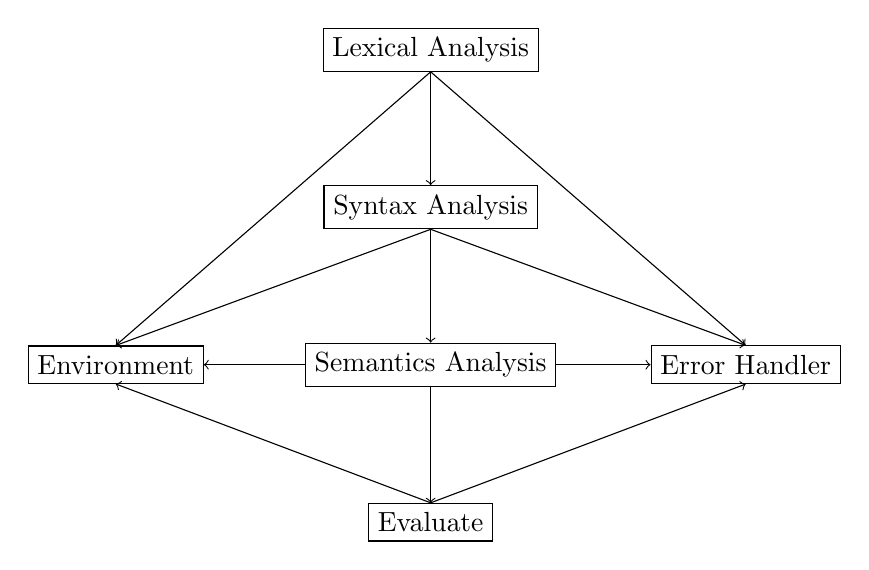
\begin{tikzpicture}
\node (la) at (4,0) [draw, rectangle] {Lexical Analysis};
\node (sa) at (4,-2) [draw, rectangle] {Syntax Analysis};
\node (err) at (8, -4) [draw, rectangle] {Error Handler};
\node (sm) at (4, -4) [draw, rectangle] {Semantics Analysis};
\node (env) at (0, -4) [draw, rectangle] {Environment};
\node (ev) at (4, -6) [draw, rectangle] {Evaluate};
\draw[->] (la.south) -- (sa.north);
\draw [->] (sa.south) -- (sm.north);
\draw [->] (sm.south) -- (ev.north);
\draw [->] (la.south) -- (env.north);
\draw [->] (la.south) -- (err.north);
\draw [->] (sa.south) -- (env.north);
\draw [->] (sa.south) -- (err.north);
\draw [->] (sm.west) -- (env.east);
\draw [->] (sm.east) -- (err.west);
\draw [->] (ev.north) -- (env.south);
\draw [->] (ev.north) -- (err.south);
\end{tikzpicture}
\caption{Interpreter phases \cite{dragonbook}}
\end{figure}
\end{frame}

\begin{frame}
\frametitle{Experience with Lexical Analysis}
\begin{figure} 
	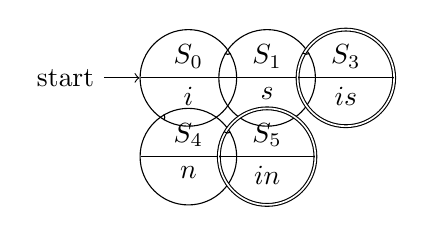
\begin{tikzpicture}
		\node[state with output, initial] (s0) {$S_0$ \nodepart{lower} $i$};
		\node[state with output, right of=s0] (s1) {$S_1$ \nodepart{lower} $s$};
		\node[state with output, accepting, right of=s1] (s2) {$S_3$ \nodepart{lower} $is$};
        \node[state with output, below of=s0] (s3){$S_4$ \nodepart{lower} $n$};
        \node[state with output, accepting, right of=s3] (s4) {$S_5$ \nodepart{lower} $in$};
		
		\draw (s0) edge[bend left] node[above]{} (s1)
			  %
			  (s1) edge[bend left] node[above]{} (s2)
                %
                (s0) edge[bend right] node[below]{} (s3)
                %
                (s3) edge[bend left] node[above]{} (s4)
        ;
	\end{tikzpicture}
    \caption{Finite State for keywords \textit{is} and \textit{in}}
\end{figure}
\end{frame}

\begin{frame}
\frametitle{Scheme}
\begin{figure}
    \centering
    \includegraphics[scale=0.45]{lisp.png}
    \caption{Lisp Mascot \cite{seasoned}}
    \label{fig:enter-label}
\end{figure}
((((((((((((((((((((((((((((((((((((((((((((((((((((((((((((((((((((((((
((((((((((((((((((((((((((((((((((((((((((((((((((((((((((((((((((((((((
((((((((((((((((((((((((((((((((((((((((((((((((((((((((((((((((((((((((
((((((((((((((((((((((((((((((((((((((((((((((((((((((((((((((((((((((((
((((((((((((((((((((((((((((((((((((((((((((((((((((((((((((((((((((((((
((((((((((((((((((((((((((((((((((((((((((((((((((((((((((((((((((((((((
\end{frame}

\begin{frame}
\frametitle{More Scheme...}
))))))))))))))))))))))))))))))))))))))))))))))))))))))))))))))))))))))))
))))))))))))))))))))))))))))))))))))))))))))))))))))))))))))))))))))))))
))))))))))))))))))))))))))))))))))))))))))))))))))))))))))))))))))))))))
))))))))))))))))))))))))))))))))))))))))))))))))))))))))))))))))))))))))
))))))))))))))))))))))))))))))))))))))))))))))))))))))))))))))))))))))))
))))))))))))))))))))))))))))))))))))))))))))))))))))))))))))))))))))))))
\end{frame}


\begin{frame}
\frametitle{Where I am at}
\begin{itemize}
    \item Completed Lexical Analysis (Scanning)
    \item Starting Syntax Analysis (Parsing)
    \item Studying Topology and Homotopy Type Theory \cite{hott}
\end{itemize}
\end{frame}

\begin{frame}
  \frametitle{What I've learned from Homotopy Type Theory}
  \begin{figure}
    \centering
    \includegraphics[scale=0.05]{socrates.jpg}
    \caption{Socrates}
    \label{fig:enter-label}
\end{figure}
    \begin{itemize}
    \item Nothing
    \item Types are paths, not objects
      \item \( (A = B) \cong (A \cong B) \)
    \end{itemize}
\end{frame}

\begin{frame}[allowframebreaks]
\frametitle{References}
\bibliographystyle{acm}
\bibliography{refs}
\end{frame}
\end{document}
%% DOC END %%
